%%%%%%%%%%%%%%%%%%%%%%%%%%%%%%%%%%%%%%%%%
% Beamer Presentation
% LaTeX Template
% Version 1.0 (10/11/12)
%
% This template has been downloaded from:
% http://www.LaTeXTemplates.com
%
% License:
% CC BY-NC-SA 3.0 (http://creativecommons.org/licenses/by-nc-sa/3.0/)
%
%%%%%%%%%%%%%%%%%%%%%%%%%%%%%%%%%%%%%%%%%

%----------------------------------------------------------------------------------------
%	PACKAGES AND THEMES
%----------------------------------------------------------------------------------------

\documentclass{beamer}

\mode<presentation> {

% The Beamer class comes with a number of default slide themes
% which change the colors and layouts of slides. Below this is a list
% of all the themes, uncomment each in turn to see what they look like.

%\usetheme{default}
%\usetheme{AnnArbor}
%\usetheme{Antibes}
%\usetheme{Bergen}
%\usetheme{Berkeley}
%\usetheme{Berlin}
%\usetheme{Boadilla}
%\usetheme{CambridgeUS}
%\usetheme{Copenhagen} --
%\usetheme{Darmstadt} --
%\usetheme{Dresden}
%\usetheme{Frankfurt} --
%\usetheme{Goettingen}
%\usetheme{Hannover}
%\usetheme{Ilmenau}
%\usetheme{JuanLesPins}
%\usetheme{Luebeck}
\usetheme{Madrid}
%\usetheme{Malmoe}
%\usetheme{Marburg}
%\usetheme{Montpellier}
%\usetheme{PaloAlto}
%\usetheme{Pittsburgh}
%\usetheme{Rochester}
%\usetheme{Singapore}
%\usetheme{Szeged}
%\usetheme{Warsaw}

% As well as themes, the Beamer class has a number of color themes
% for any slide theme. Uncomment each of these in turn to see how it
% changes the colors of your current slide theme.

%\usecolortheme{albatross}
%\usecolortheme{beaver}
%\usecolortheme{beetle}
%\usecolortheme{crane}
%\usecolortheme{dolphin}
%\usecolortheme{dove}
%\usecolortheme{fly}
%\usecolortheme{lily}
%\usecolortheme{orchid}
%\usecolortheme{rose}
%\usecolortheme{seagull}
%\usecolortheme{seahorse}
%\usecolortheme{whale}
%\usecolortheme{wolverine}

%\setbeamertemplate{footline} % To remove the footer line in all slides uncomment this line
%\setbeamertemplate{footline}[page number] % To replace the footer line in all slides with a simple slide count uncomment this line

%\setbeamertemplate{navigation symbols}{} % To remove the navigation symbols from the bottom of all slides uncomment this line
}

\usepackage[spanish]{babel}
\usepackage[utf8]{inputenc}

\usepackage{graphicx} % Allows including images
\usepackage{booktabs} % Allows the use of \toprule, \midrule and \bottomrule in tables

\usepackage{subcaption}
\captionsetup{compatibility=false}

\renewcommand\footnotemark{}
\renewcommand\footnoterule{}

\usepackage[export]{adjustbox}
\usepackage{wrapfig}

\usepackage{textpos}

\newenvironment{figure*}%
{\begin{figure}}
{\end{figure}}

%----------------------------------------------------------------------------------------
%	TITLE PAGE
%----------------------------------------------------------------------------------------

\title[RRAP]{Proyecto de grado: Routers Reconfigurables de Altas Prestaciones} % The short title appears at the bottom of every slide, the full title is only on the title page

\author{Rodrigo Amaro, Emiliano Viotti}
\institute[UdelaR] % Your institution as it will appear on the bottom of every slide, may be shorthand to save space
{
Instituto de Computaci\'on \\ Facultad de Ingeniería \\ Universidad de la República \\ \vspace{0.2cm} Tutores: Dr. Eduardo Gramp\'in, MSc. Mart\'in Giachino % Your institution for the title page
%\medskip
%\textit{john@smith.com} % Your email address
}
\date{\today} % Date, can be changed to a custom date

\begin{document}

\begin{frame}
\titlepage % Print the title page as the first slide
\end{frame}


\begin{frame}
\frametitle{Agenda} % Table of contents slide, comment this block out to remove it
\tableofcontents % Throughout your presentation, if you choose to use \section{} and \subsection{} commands, these will automatically be printed on this slide as an overview of your presentation
\end{frame}

%----------------------------------------------------------------------------------------
%	PRESENTATION SLIDES
%----------------------------------------------------------------------------------------


%------------------------------------------------
\section{Motivaci\'on} 

\begin{frame}
\frametitle{Motivaci\'on} 

\begin{block}{Redes acad\'emicas}
Internet no parece apropiada para su utilizaci\'on en el contexto académico en el desarrollo de nuevos protocolos y servicios, investigaci\'on y la innovaci\'on en el \'area.
\end{block}

\begin{figure}[h] 
\centering    
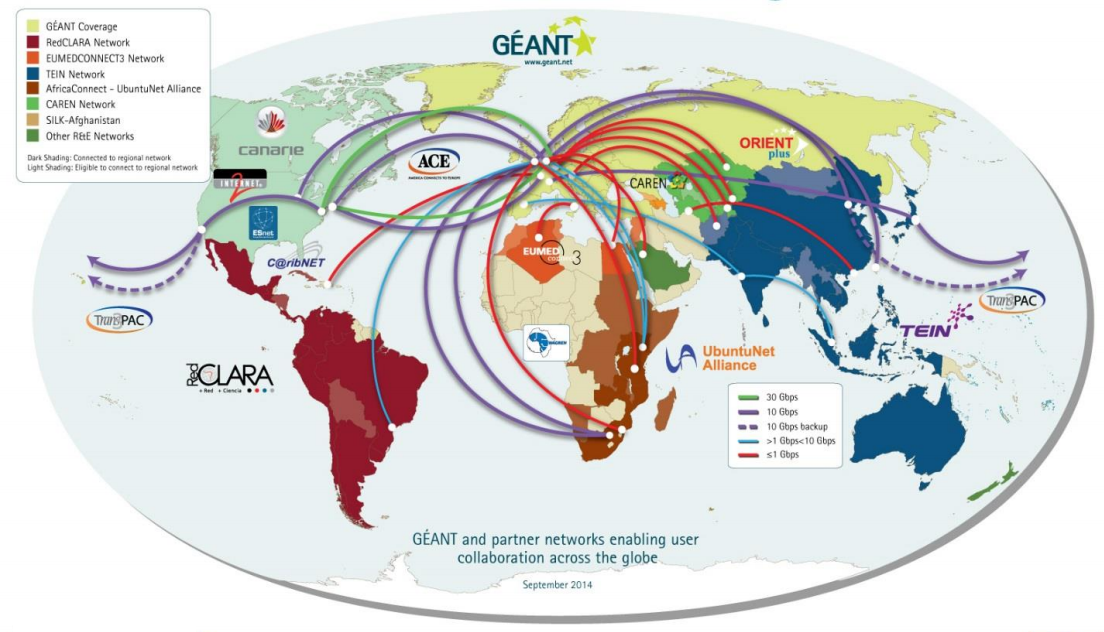
\includegraphics[width=0.7\textwidth]{imagenes/redesAcademicas.png}
\label{fig:AcademicNetworks}
\end{figure}

\end{frame}

\begin{frame}
\frametitle{Motivaci\'on} 

\begin{block}{Red Académica Uruguaya (RAU)}
A nivel local, la RAU es un emprendimiento de la Universidad de la República administrado por el SeCIU con los objetivos de unir a las instituciones académicas nacionales en una red de alcance nacional y a trav\'es de ella conectarlas a Latinoam\'erica. 
\end{block}

\begin{block}{RAU2}
Remplazo de la actual red académica, es una red avanzada de altas prestaciones que estar\'ia dotada de funciones de virtualizaci\'on de redes flexibles en su definici\'on y uso.
\end{block}

\begin{figure}[h] 
\centering    

\includegraphics[width=0.3\textwidth]{imagenes/logorau2.png}
\label{fig:RAU}
\end{figure}

\end{frame}

\begin{frame}
\frametitle{Motivaci\'on} 

\begin{block}{Hardware comercial}
Los equipos de red de backbone comerciales como HP, CISCO, Juniper son costos y generalmente de naturaleza cerrada. Las funcionalidades del hardware se restringen a las funcionalidades expuesta por
una API propietaria. 
\end{block}

\begin{figure}[htp]
\centering
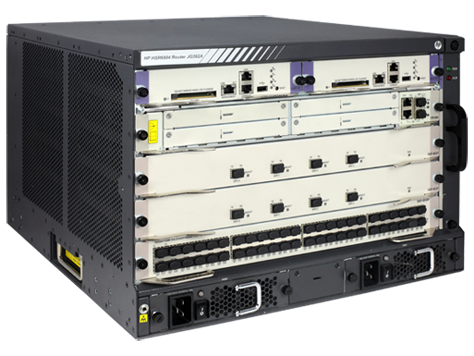
\includegraphics[width=.25\textwidth]{imagenes/corerouter2.png}\hfill
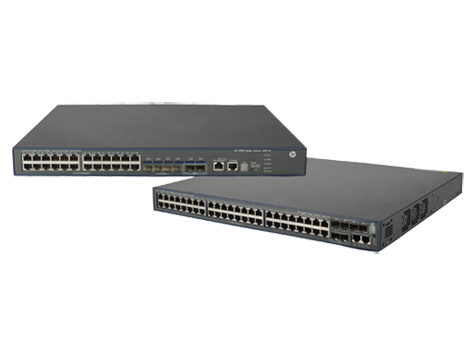
\includegraphics[width=.35\textwidth]{imagenes/corerouter1.png}\hfill
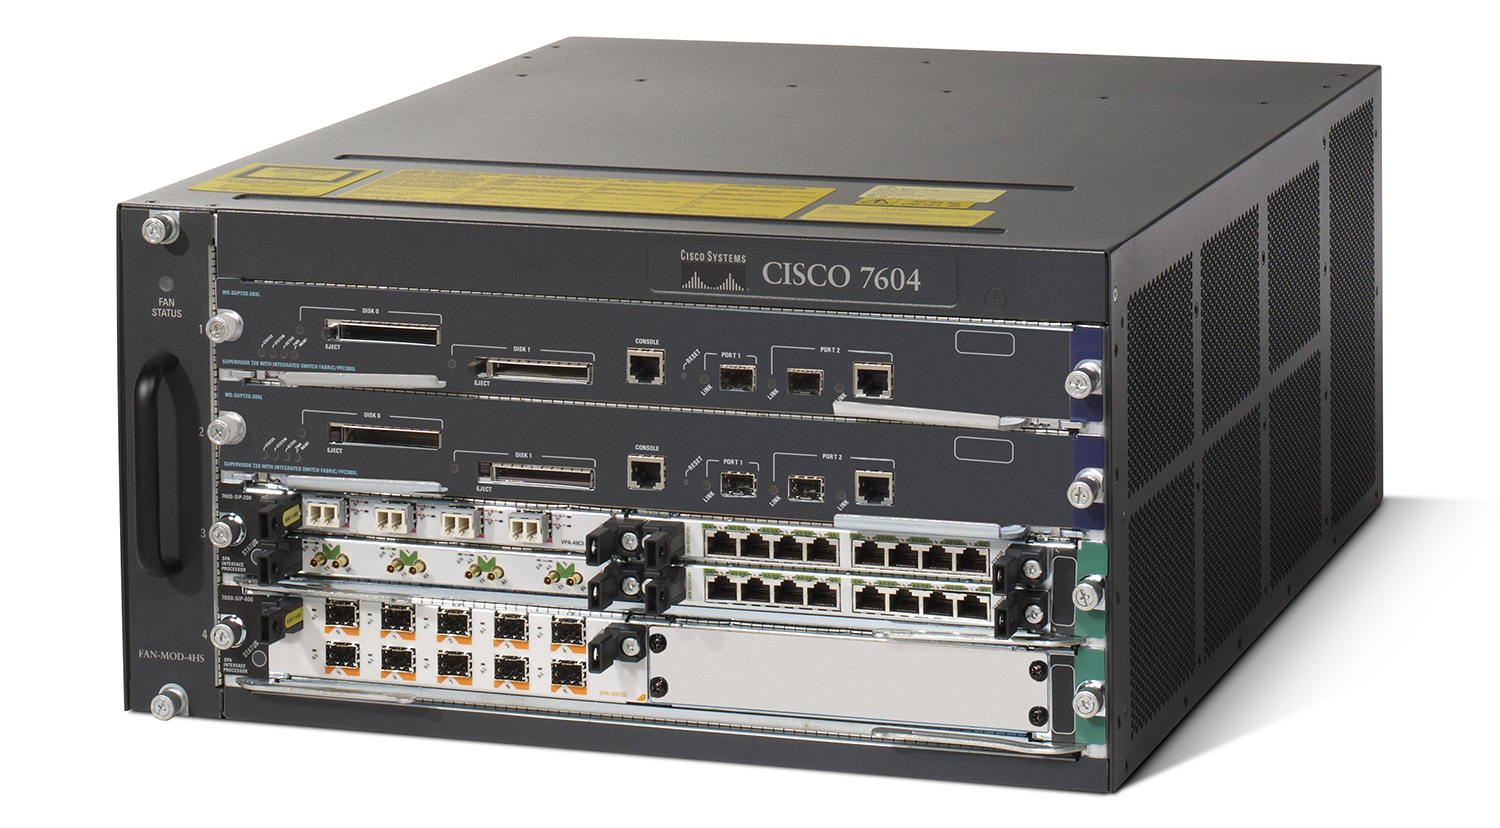
\includegraphics[width=.35\textwidth]{imagenes/corerouter3.jpg}
\label{fig:figure3}
\end{figure}
\end{frame}
%------------------------------------------------

%------------------------------------------------
\section{Definición del problema} 


\begin{frame}
\frametitle{Definición del problema} 

\begin{block}{Definición del Problema }
Constru\'ir un prototipo para la RAU2 utilizando como plataforma PCs con placas de red aceleradas en hardware reconfigurable NetFPGA y el enfoque de las Redes Definidas por Software (SDN).

\end{block}
\end{frame}

\begin{frame}
\frametitle{Definición del problema} 

\begin{block}{Objetivos}
Enumerar los principales objetivos
\end{block}

\begin{block}{Resultados esperados}
\begin{itemize}
\item Estado del arte en Redes Definidas por Software y hardware NetFPGA
\item Prototipo de aplicaci\'on de gesti\'on de red utilizando SDN y el hardware NetFPGA enfocado en los requerimientos recabados sobre la RAU2
\item Diseño e implementaci\'on de pruebas de verificaci\'on para el prototipo construido
\end{itemize}
\end{block}

\end{frame}

%------------------------------------------------

%------------------------------------------------
\section{Conceptos preliminares} 


\begin{frame}
\frametitle{SDN-Enfoque tradicional} 


SDN Es un enfoque arquitectonico alternativo al enfoque tradicional de redes.

Enfoque tradicional:

PHOTO

\begin{block}{Enfoque tradicional}
La inteligencia y estado de la red se encuentra distribuida en los mismos dispositivos que reenvian la informacion
\end{block}
%Imagen enfoque tradicional


\end{frame}

\begin{frame}
\frametitle{SDN-Plano de control y plano de datos} 


\begin{block}{Plano de control}

El plano de control donde reside la inteligencia de la red... robar de CRA
\end{block}
ejemplos son: algoritmos de ruteo tradicionales, OSPF, RIP,Firewalls


\begin{block}{Plano de datos}
\end{block}



%Imagen enfoque tradicional

\end{frame}

\begin{frame}
\frametitle{SDN} 
Definicion:
Y mostrar imagen enfoque tradicional vs sdn

\end{frame}


%SDN 
%
%PUNTO DE CONTROL CENTRALIZADO DE LA RED
%BUSCAR OTROS EJEMPLOS DE implementaciones SDN
%
%EJEMPLOS DE PLANO DE CONTROL, ospfd, firewalls etc
%
%
%Alternativa al enfoque tradicional
%EN SDN MOSTRAR UNA IMAGEN DE ARQUITECTURA ACTUAL Y 
%ARQUITECTURA SDN
%Pueden ser parecidas a esto:
%http://millennialmainframer.com/2012/09/the-mainframe-and-software-defined-networking/
%http://www.aryaka.com/why-sdn-concepts-need-to-extend-into-the-wan/
%
%
%Es una solucion abierta de SDN
%
%Define una arquitectura
%
%
%-----Elegir una imagen que muestre las apps arriba del controler
% y explicar como se programa------
%COntrolador
%(Interfaz sur
%Interfaz norte
%Interfaz este-oeste)
%Protocolo
%Dispositivo opewnflow-capable(Canal openflow, tablas)
%----------------------
%
%Define un protocolo y una estructura de mensaje
%
%
%Define un protocolo de red que permite comunicar el controlador(plano de control) 
%con los dispositivos (plano de datos)
%Rapido hablar de los tres tipos de mensajes(Controlador a disp,asinc, simetricos(keepalives,echos))
%
%Define la estructura de la tabla de flujos
%
%(Match field)
%Que match fields? Mostrar una imagen con ether, mpls tpc ip
%
%(Contador, estadisticas por flujo)
%Instrucciones(Que hacer? reenviar ,modificar y reenviar, broadcast, multicast, normal).
%
%
%Ventajas y desventajas?



\begin{frame}
\frametitle{OpenFlow} 
Solucion basada en el enfoque SDN


\end{frame}

\begin{frame}
\frametitle{OpenFlow} 
1 Transicion) Controlador o sistema operativo de red.(Plano de control) 
/*
Llamado el sistema operativo de la red, 
*/
Software que ejecuta en hardware x86 (PC, Servidor)
Ofrece una api de alto nivel a los programadores (NorthBound) para controlar la red.
Cada operacion ofrecida por la api es traducida a reglas openflow y comunicadas por el canal openflow (SouthBound)hacia el dispositivo.
\end{frame}

\begin{frame}
\frametitle{OpenFlow} 

2 Transicion) Canal Openflow 
Entre el controlador y los dispositivos
Protocolo OpenFlow
Capa de aplicacion, corre sobre TCP

Define mensajes
- Controlador a dispositivo. 
- Asincronicos
- Simetricos (keepalives,echos)

\end{frame}

\begin{frame}
\frametitle{OpenFlow} 
Dispositivo:

Dispositivo opewnflow-capable(Canal openflow, tablas)


Canal openflow

Tabla en un dispositivo:    
/*
Cabe destacar que mediante firmware.... uno de los porque del exito de openflow..
*/

(Match field, mostrar imagen famosa)
(Contador, estadisticas por flujo)
Instrucciones(Que hacer? reenviar ,modificar y reenviar, broadcast, multicast, normal).
\end{frame}

\begin{frame}
\frametitle{VPN} 

\end{frame}

\begin{frame}
\frametitle{MPLS} 

\end{frame}


\begin{frame}
\frametitle{NetFPGA} 


	Plataforma de hardware de red reconfigurable y software OpenSource.



%	\begin{block}{Hardware}
		Hardware: Placa PCI-E que cuenta con: 
		\begin{enumerate}
			\item Chip programable FPGA 
			\item 15 GB RAM
			\item 4 Puertos 10-Gigabit Ethernet
		\end{enumerate}
		
	\begin{figure}[H]
		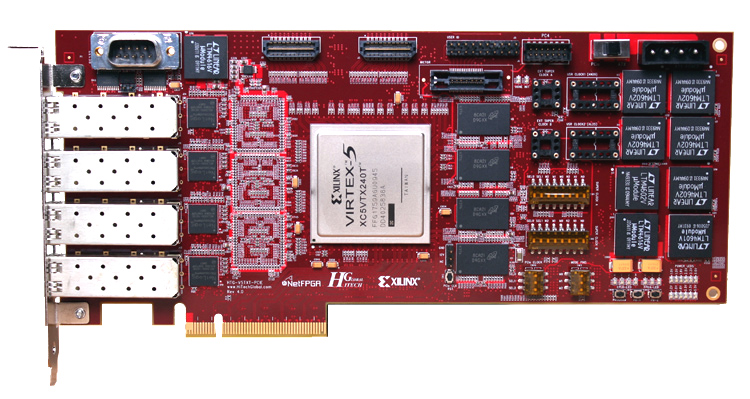
\includegraphics[width=0.65\textwidth, right]{imagenes/NetFPGA10G_web.jpg}
	\end{figure}

%	\end{block}

\end{frame}




\begin{frame}
\frametitle{NetFPGA} 
\begin{block}{Software}
Proyectos de software OpenSource que permiten programar comportamientos de la placa

\begin{enumerate}
\item Router IP
\item Switch Ethernet
\item Placa de red convencional
\item Switch OpenFlow 1.0
\end{enumerate}

\end{block}

\end{frame}







%------------------------------------------------
\section{Arquitectura de la soluci\'on} 

\begin{frame}
\frametitle{Arquitectura de la soluci\'on} 

Poner una imagen de la arquitectura esperada basada en SDN
plano de control, plano de datos dispositivos OpenFlow capaz, etc. Mi idea es ahi explicar
las cuestiones que hay que atacar. En el trabajo hay que implementar:
1) Plano de Control
2) Dispisitivos SDN/OpenFlow

Redondear ambas lineas de trabajo mientras se explica asi se pasa en las siguientes ppt a hablar de eso

\end{frame}

\begin{frame}
\frametitle{Arquitectura de la soluci\'on} 

\textbf{Construir un switch OpenFlow} 

\vspace{0.3cm}
Se identifican dos alternativas: 
\begin{enumerate}
\item Proyecto OpenFlow
\item Proyecto ReferenceNIC m\'as implementaci\'on OF en software (Open vSwitch)
\end{enumerate}

\begin{table}[]
\small
\centering
\label{label}
\begin{tabular}{| p{5cm} | p{5cm} |}

\hline
\multicolumn{1}{|c|}{(1) OpenFlow } & \multicolumn{1}{c|}{(2) ReferenceNIC y OvS } \\
\hline
Velocidad de procesamiento & Prototipaci\'on agil \\
Utilizaci\'on del hardaware &  Tiempo libre para investigaci\'on \\
Conocimiento espec\'ifico &  No hay que utilizar HDLs \\
Licencias full &  Licencias econ\'omicas \\

\hline  
\end{tabular}
\end{table}

\end{frame}


\begin{frame}
\frametitle{Arquitectura de la soluci\'on} 

\begin{minipage}{0.60\textwidth}
Switch OpenFlow

Dos alternativas: Mencionarlas (NetFPGA + Openflow, ...)

Mostrar las dos fotos del stack Plano Control - Dispositivo con los building blocks

\end{minipage}
\hfill
\begin{minipage}{0.30\textwidth}
\begin{figure}[H]
\raggedright
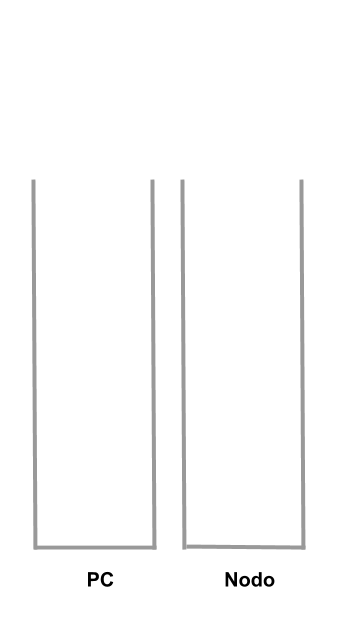
\includegraphics[width=1.0\textwidth, right]{imagenes/Stack.png}
\end{figure}
\end{minipage} 

\pause

\begin{textblock}{3}(11.47,-2.9)
\begin{minipage}{\textwidth}
\setlength{\parindent}{0pt}
\setlength{\parskip}{0.1cm}
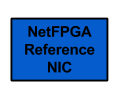
\includegraphics[width=0.53\textwidth, right]{imagenes/buildingbnetfpga.png}
\end{minipage}
\end{textblock}

\begin{textblock}{3}(11.47,-4.2)
\begin{minipage}{\textwidth}
\setlength{\parindent}{0pt}
\setlength{\parskip}{0.1cm}
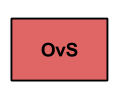
\includegraphics[width=0.53\textwidth, right]{imagenes/buildingblockovs.png}
\end{minipage}
\end{textblock}

\end{frame}

\begin{frame}
\frametitle{Arquitectura de la soluci\'on} 


\begin{minipage}{0.60\textwidth}
Controlador

Utilizamos Ryu blablabla....

Mostrar las dos fotos del stack Plano Control - Dispositivo con los building blocks

\end{minipage}
\hfill
\begin{minipage}{0.30\textwidth}
\begin{figure}[H]
\raggedright
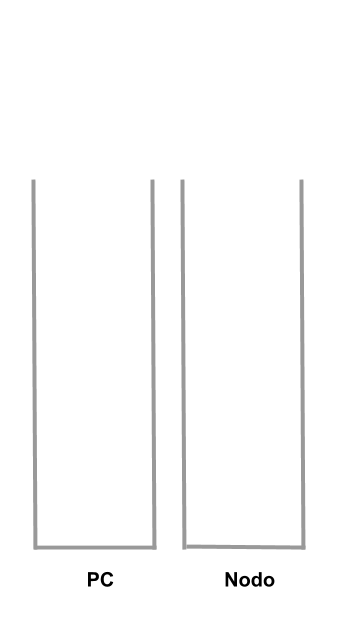
\includegraphics[width=1.0\textwidth, right]{imagenes/Stack.png}
\end{figure}
\end{minipage} 

\begin{textblock}{3}(11.47,-2.9)
\begin{minipage}{\textwidth}
\setlength{\parindent}{0pt}
\setlength{\parskip}{0.1cm}
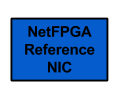
\includegraphics[width=0.53\textwidth, right]{imagenes/buildingbnetfpga.png}
\end{minipage}
\end{textblock}

\begin{textblock}{3}(11.47,-4.2)
\begin{minipage}{\textwidth}
\setlength{\parindent}{0pt}
\setlength{\parskip}{0.1cm}
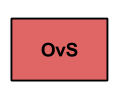
\includegraphics[width=0.53\textwidth, right]{imagenes/buildingblockovs.png}
\end{minipage}
\end{textblock}

\pause

\begin{textblock}{3}(9.55,-2.9)
\begin{minipage}{\textwidth}
\setlength{\parindent}{0pt}
\setlength{\parskip}{0.1cm}
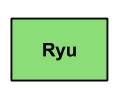
\includegraphics[width=0.53\textwidth, right]{imagenes/buildingblockryu.png}
\end{minipage}
\end{textblock}

\end{frame}

\begin{frame}
\frametitle{Arquitectura de la soluci\'on} 

\begin{minipage}{0.60\textwidth}
\onslide<1->{Algoritmo de ruteo}

\onslide<2->{OSPF para el descubrimiento de la topologia y algoritmo de ruteo centralizado

Mostrar las dos fotos del stack Plano Control - Dispositivo con los building blocks}

\end{minipage}
\hfill
\begin{minipage}{0.30\textwidth}
\begin{figure}[H]
\raggedright
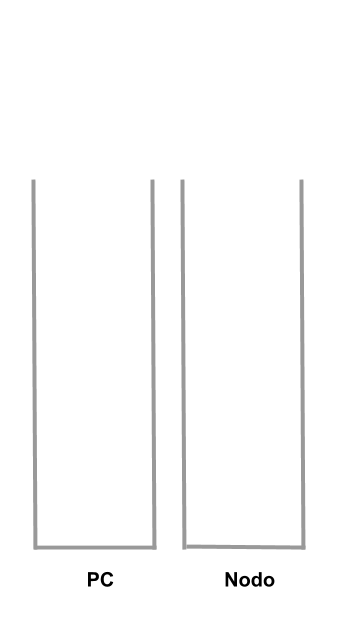
\includegraphics[width=1.0\textwidth, right]{imagenes/Stack.png}
\end{figure}
\end{minipage} 

\begin{textblock}{3}(11.47,-2.9)
\begin{minipage}{\textwidth}
\setlength{\parindent}{0pt}
\setlength{\parskip}{0.1cm}
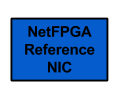
\includegraphics[width=0.53\textwidth, right]{imagenes/buildingbnetfpga.png}
\end{minipage}
\end{textblock}

\begin{textblock}{3}(11.47,-4.2)
\begin{minipage}{\textwidth}
\setlength{\parindent}{0pt}
\setlength{\parskip}{0.1cm}
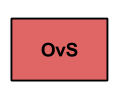
\includegraphics[width=0.53\textwidth, right]{imagenes/buildingblockovs.png}
\end{minipage}
\end{textblock}

\begin{textblock}{3}(9.55,-2.9)
\begin{minipage}{\textwidth}
\setlength{\parindent}{0pt}
\setlength{\parskip}{0.1cm}
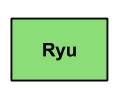
\includegraphics[width=0.53\textwidth, right]{imagenes/buildingblockryu.png}
\end{minipage}
\end{textblock}

\pause

\begin{textblock}{3}(11.47,-5.5)
\begin{minipage}{\textwidth}
\setlength{\parindent}{0pt}
\setlength{\parskip}{0.1cm}
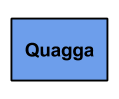
\includegraphics[width=0.53\textwidth, right]{imagenes/buildingblockquagga.png}
\end{minipage}
\end{textblock}

\begin{textblock}{3}(9.55,-4.2)
\begin{minipage}{\textwidth}
\setlength{\parindent}{0pt}
\setlength{\parskip}{0.1cm}
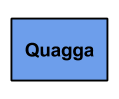
\includegraphics[width=0.53\textwidth, right]{imagenes/buildingblockquagga.png}
\end{minipage}
\end{textblock}

\end{frame}

\begin{frame}
\frametitle{Arquitectura de la soluci\'on} 

\begin{minipage}{0.60\textwidth}
RAUFlow App algoritmo de ruteo, clasificacion de trafico, LDP etc
\end{minipage}
\hfill
\begin{minipage}{0.30\textwidth}
\begin{figure}[H]
\raggedright
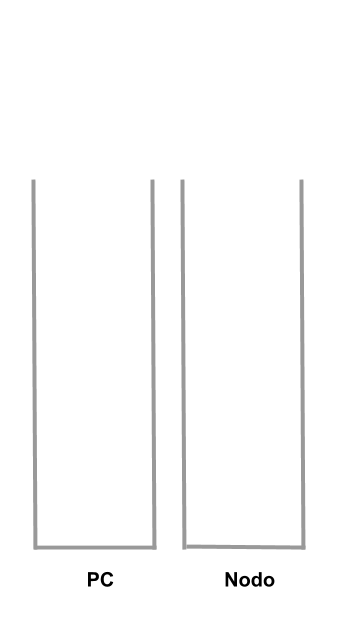
\includegraphics[width=1.0\textwidth, right]{imagenes/Stack.png}
\end{figure}
\end{minipage} 

\begin{textblock}{3}(11.47,-2.9)
\begin{minipage}{\textwidth}
\setlength{\parindent}{0pt}
\setlength{\parskip}{0.1cm}
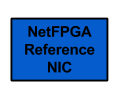
\includegraphics[width=0.53\textwidth, right]{imagenes/buildingbnetfpga.png}
\end{minipage}
\end{textblock}

\begin{textblock}{3}(11.47,-4.2)
\begin{minipage}{\textwidth}
\setlength{\parindent}{0pt}
\setlength{\parskip}{0.1cm}
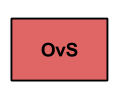
\includegraphics[width=0.53\textwidth, right]{imagenes/buildingblockovs.png}
\end{minipage}
\end{textblock}

\begin{textblock}{3}(9.55,-2.9)
\begin{minipage}{\textwidth}
\setlength{\parindent}{0pt}
\setlength{\parskip}{0.1cm}
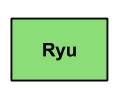
\includegraphics[width=0.53\textwidth, right]{imagenes/buildingblockryu.png}
\end{minipage}
\end{textblock}

\begin{textblock}{3}(11.47,-5.5)
\begin{minipage}{\textwidth}
\setlength{\parindent}{0pt}
\setlength{\parskip}{0.1cm}
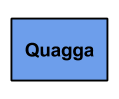
\includegraphics[width=0.53\textwidth, right]{imagenes/buildingblockquagga.png}
\end{minipage}
\end{textblock}

\begin{textblock}{3}(9.55,-4.2)
\begin{minipage}{\textwidth}
\setlength{\parindent}{0pt}
\setlength{\parskip}{0.1cm}
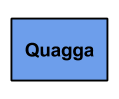
\includegraphics[width=0.53\textwidth, right]{imagenes/buildingblockquagga.png}
\end{minipage}
\end{textblock}

\pause

\begin{textblock}{3}(9.55,-5.5)
\begin{minipage}{\textwidth}
\setlength{\parindent}{0pt}
\setlength{\parskip}{0.1cm}
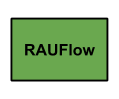
\includegraphics[width=0.53\textwidth, right]{imagenes/buldingblockrauflow.png}
\end{minipage}
\end{textblock}


\end{frame}

\begin{frame}
\frametitle{Arquitectura de la soluci\'on} 

\begin{minipage}{0.60\textwidth}
Mapeo de puertos a direcciones IP

SNMP

Mostrar las dos fotos del stack Plano Control - Dispositivo con los building blocks
\end{minipage}
\hfill
\begin{minipage}{0.30\textwidth}
\begin{figure}[H]
\raggedright
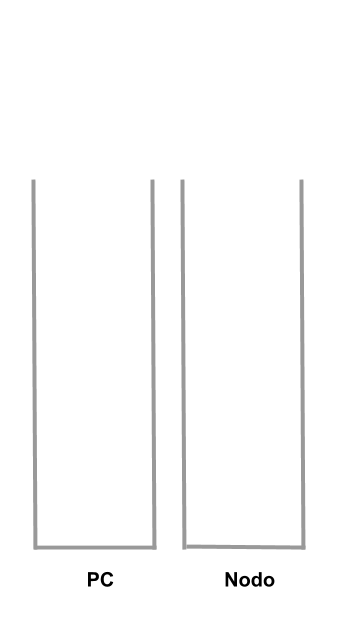
\includegraphics[width=1.0\textwidth, right]{imagenes/Stack.png}
\end{figure}
\end{minipage} 

\begin{textblock}{3}(11.47,-2.9)
\begin{minipage}{\textwidth}
\setlength{\parindent}{0pt}
\setlength{\parskip}{0.1cm}
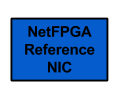
\includegraphics[width=0.53\textwidth, right]{imagenes/buildingbnetfpga.png}
\end{minipage}
\end{textblock}

\begin{textblock}{3}(11.47,-4.2)
\begin{minipage}{\textwidth}
\setlength{\parindent}{0pt}
\setlength{\parskip}{0.1cm}
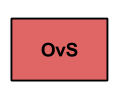
\includegraphics[width=0.53\textwidth, right]{imagenes/buildingblockovs.png}
\end{minipage}
\end{textblock}

\begin{textblock}{3}(9.55,-2.9)
\begin{minipage}{\textwidth}
\setlength{\parindent}{0pt}
\setlength{\parskip}{0.1cm}
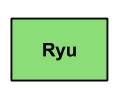
\includegraphics[width=0.53\textwidth, right]{imagenes/buildingblockryu.png}
\end{minipage}
\end{textblock}

\begin{textblock}{3}(11.47,-5.5)
\begin{minipage}{\textwidth}
\setlength{\parindent}{0pt}
\setlength{\parskip}{0.1cm}
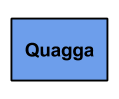
\includegraphics[width=0.53\textwidth, right]{imagenes/buildingblockquagga.png}
\end{minipage}
\end{textblock}

\begin{textblock}{3}(9.55,-4.2)
\begin{minipage}{\textwidth}
\setlength{\parindent}{0pt}
\setlength{\parskip}{0.1cm}
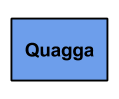
\includegraphics[width=0.53\textwidth, right]{imagenes/buildingblockquagga.png}
\end{minipage}
\end{textblock}

\begin{textblock}{3}(9.55,-5.5)
\begin{minipage}{\textwidth}
\setlength{\parindent}{0pt}
\setlength{\parskip}{0.1cm}
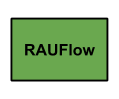
\includegraphics[width=0.53\textwidth, right]{imagenes/buldingblockrauflow.png}
\end{minipage}
\end{textblock}

\pause

\begin{textblock}{3}(9.55,-6.8)
\begin{minipage}{\textwidth}
\setlength{\parindent}{0pt}
\setlength{\parskip}{0.1cm}
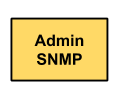
\includegraphics[width=0.53\textwidth, right]{imagenes/buildingblockadminsnmp.png}
\end{minipage}
\end{textblock}

\begin{textblock}{3}(11.47,-6.8)
\begin{minipage}{\textwidth}
\setlength{\parindent}{0pt}
\setlength{\parskip}{0.1cm}
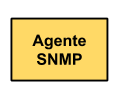
\includegraphics[width=0.53\textwidth, right]{imagenes/buildingblockagentesnmp.png}
\end{minipage}
\end{textblock}
\end{frame}

%------------------------------------------------

%------------------------------------------------
\section{Implementaci\'on} 

\begin{frame}
\frametitle{Implementaci\'on} 

\end{frame}
%------------------------------------------------

%------------------------------------------------
\section{Conclusiones} 

\begin{frame}
\frametitle{Conclusiones} 

\begin{itemize}
\item Se realiz\'o una investigaci\'on en profundidad del estado del arte de las redes definidas por software (SDN) y la plataforma de hardware NetFPGA

\item Se implement\'o un prototipo de red de backbone utilizando el hardware NetFPGA y el enfoque SDN

\item Se implement\'o un conjunto de pruebas para la verificaci\'on del prototipo construido 

\end{itemize}
\end{frame}

\begin{frame}
\frametitle{Conclusiones} 

\begin{itemize}
\item Se realiz\'o una investigaci\'on en profundidad del estado del arte de las redes definidas por software (SDN) y la plataforma de hardware NetFPGA
\end{itemize}

\end{frame}


\begin{frame}
\frametitle{Conclusiones} 

Se implement\'o un prototipo de red de backbone utilizando el hardware NetFPGA y el enfoque SDN:

\begin{itemize}
\item \textbf{RAUswitch} Se construy\'o un router de backbone IP/MPLS compatible con el protocolo OpenFlow y OSPF utilizando el hardware NetFPGA

\item \textbf{RAUflow} Se implement\'o una aplicaci\'on de gesti\'on de red utilizando el enfoque SDN con funcionalidades para la definici\'on de redes privadas virtuales

\begin{itemize}
\item Redefinici\'on del concepto de FEC
\item Clasificaci\'on de tr\'afico mediante protocolo OpenFlow 1.3.1
\item Algoritmo de ruteo din\'amico SPF centralizado
\end{itemize}
\end{itemize}

\end{frame}

\begin{frame}
\frametitle{Conclusiones} 

Se construy\'o un laboratorio de pruebas para la verificaci\'on del prototipo:

\begin{itemize}
\item Se verific\'o algoritmo de ruteo, distribuci\'on de etiquetas y clasificaci\'on de tr\'afico 

\item Se implement\'o el caso de uso VPN L3 Multipunto en un escenario de dos organizaciones con dos sucursales

\item Se implement\'o el caso de uso VPN L2 Punto a Punto 

\end{itemize}

\end{frame}

\begin{frame}
\frametitle{Conclusiones} 

\begin{itemize}
\item Se confeccion\'o un manual para la construcci\'on del dispositivo RAUswitch

\item Se contribuy\'o a la comunidad NetFPGA reportando dos BUGs

\item Se escribió el articulo cient\'ifico el cual fue aceptado en la conferencia Latin American Network Operations and Management Symposium (LANOMS) 2015

\item Se gener\'o un grupo de trabajo (GT SDNUY) uniendo profesionales del SeCIU, Centro de Capacitación y Desarrollo de ANTEL y del Centro Universitario de la Región Este (CURE) 

\end{itemize}

\end{frame}

%Se implement ́o un prototipo de red de backbone utilizando el
%hardware NetFPGA y el enfoque SDN
%Se implement ́o un conjunto de pruebas para la verificaci ́on del
%prototipo construido

%------------------------------------------------

%------------------------------------------------
\section{Trabajo a futuro} 

\begin{frame}
\frametitle{Trabajo a futuro} 

Se identifican las siguientes l\'ineas de trabajo a futuro:

\begin{itemize}

\item Extender el proyecto OpenFlow de la plataforma NetFPGA para soportar al menos la versi\'on 1.3.1 del protocolo OpenFlow

\item Extender el algoritmo de ruteo SPF para implementar un CSPF

\item Incorporar en RAUFlow la capacidad de soportar m\'ultiples caminos para un mismo Servicio,  balanceo de carga, QoS e Ingenier\'ia de tr\'afico

\end{itemize}

\end{frame}

\begin{frame}
\frametitle{Trabajo a futuro} 

Otras posibles l\'ineas:

\begin{itemize}

\item Agregar una capa de persistencia para ciertos datos

\item Investigar la escalabilidad de RAUflow en topolog\'ias de red realistas 

\item Construir una jerarqu\'ia de controladores e investigar el impacto en el rendimiento 

\item Incorporar m\'as dimensiones a la definici\'on de un servicio (tiempo)

\end{itemize}

\end{frame}

%------------------------------------------------

%----------------------------------------------------------------------------------------

\end{document} 

